%% EXERCICIOS PARA INCLUÍR DENTRO DO CADERNO DE EXERCICIOS %%
%
% EXERCICIO DE TRANSCRICIÓN: Epitafio de Seikilos.
%
\section{A notación musical na Antiga Grecia}


Dentro das fontes conservadas da cultura musical grega, existen aproximadamente sobre uns vinte exemplos, malia que tan só uns poucos son considerados realmente fiables, en parte debido a que a maioría deles non se conservan na súa totalidade. 

O máis destacable é un fragmento da obra de \textit{Orestes}, de Eurípides do 250 a.C., aproximadamente. Trátase dun \textit{stasimon}, isto é, un coro cantado na \textit{orchestra} (lugar diante do escenario, onde se colocaban algúns dos participantes na traxedia). A conservación é realmente boa, a pesares de non ser perfecta debido a que foi escrito en papiro e algunhas das partes perdéronse.

\subsection*{O Epitafio de Seikilos}

A fonte de información da cultura grega de maior importancia que se conserva, e que máis información aporta, é o \textit{skolion} (epitafio) de Seikilos, do século II a.C. aproximadamente. Escrito en pedra (nunha estela funeraria da actual Turquía conservado en Dinamarca), presenta unha magnífica conservación que permitiu descifralo totalmente. Podemos afirmar que é a obra máis coñecida da Antiga Grecia.

\subsubsection*{O texto}

Inscrita nunha columna (estela funeraria), serviu de epitafio a unha muller: na dedicatoria, Seikilos ofrece a unha muller (probablemente a súa esposa ou filla) unha canción, que aparece con notación musical e texto:

\begin{figure}[htp]
\centering
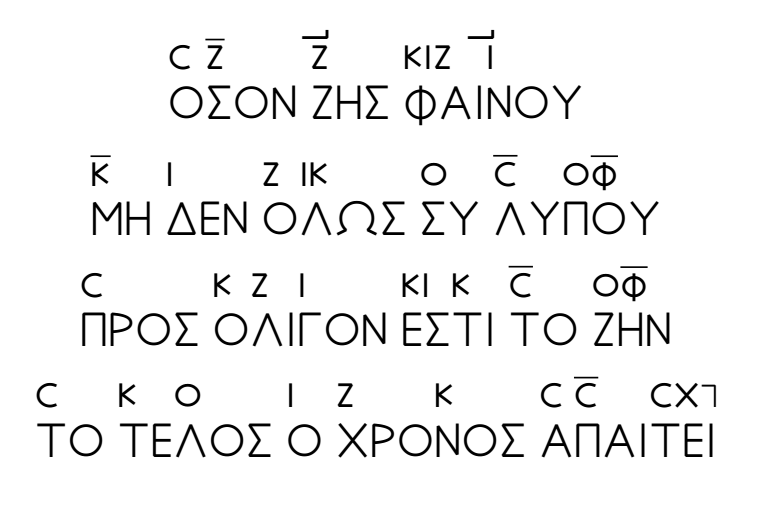
\includegraphics[scale=1.00]{images/Seikilos-Ejercicio-03.png}
\caption{Texto do epitafio de Seikilos}
\label{Seikilos-texto}
\end{figure}

A tradución sería algo semellante a: \textit{ Mentres vivas, brilla; que nada te faga sufrir; a vida é moi curta e o tempo marca a fin.}

A achega máis destacable ou importante deste documento histórico aos estudos da música grega, foi sen dúbida a notación rítmica, que ao igual que a melódica, emprega signos do alfabeto grego. As notas sen indicación rítmica, valerían un pulso (\textit{chronos protos}), as sinaladas cun guión terían dous pulsos (\textit{diseme}); finalmente, as que levan guión cun sinal ou punto na parte superior dereita valerían tres pulsos (*\textit{triseme}).

\subsubsection*{A notación musical}

\begin{itemize}
\item Para indicar a altura dos sons, empregábase un signo diferente segundo cada altura. Os signos que aparecen nesta peza, ordenados de xeito ascendente son:

	\begin{figure}[htp]
	\centering
	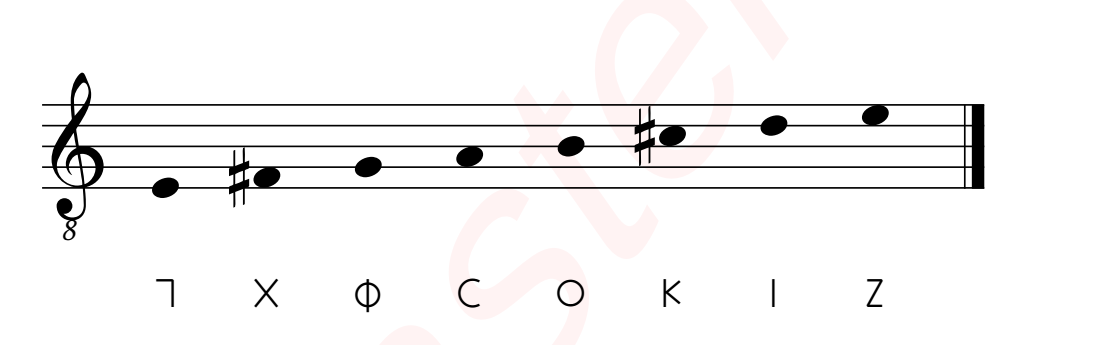
\includegraphics[scale=1.00]{images/Seikilos-Ejercicio-01.png}
	\caption{Sitema de notación}
	\label{seikilos-sistema}
	\end{figure}
	
\item Para indicar a duración, empregábanse uns signos adicionais sobre os anteriores:
	\begin{figure}[htp]
	\centering
	
\includegraphics[scale=1.00]{images/Seikilos-Ejercicio-02.png}
	\caption{Indicación da duración}
	\label{seikilos-duracion}
	\end{figure}
	
\end{itemize}

\subsubsection*{Transcrición}

Tendo en conta o indicado ata o de agora, realiza unha transcrición á notación actual da melodía do epitafio de Seikilos.

\begin{figure}[htp]
\centering
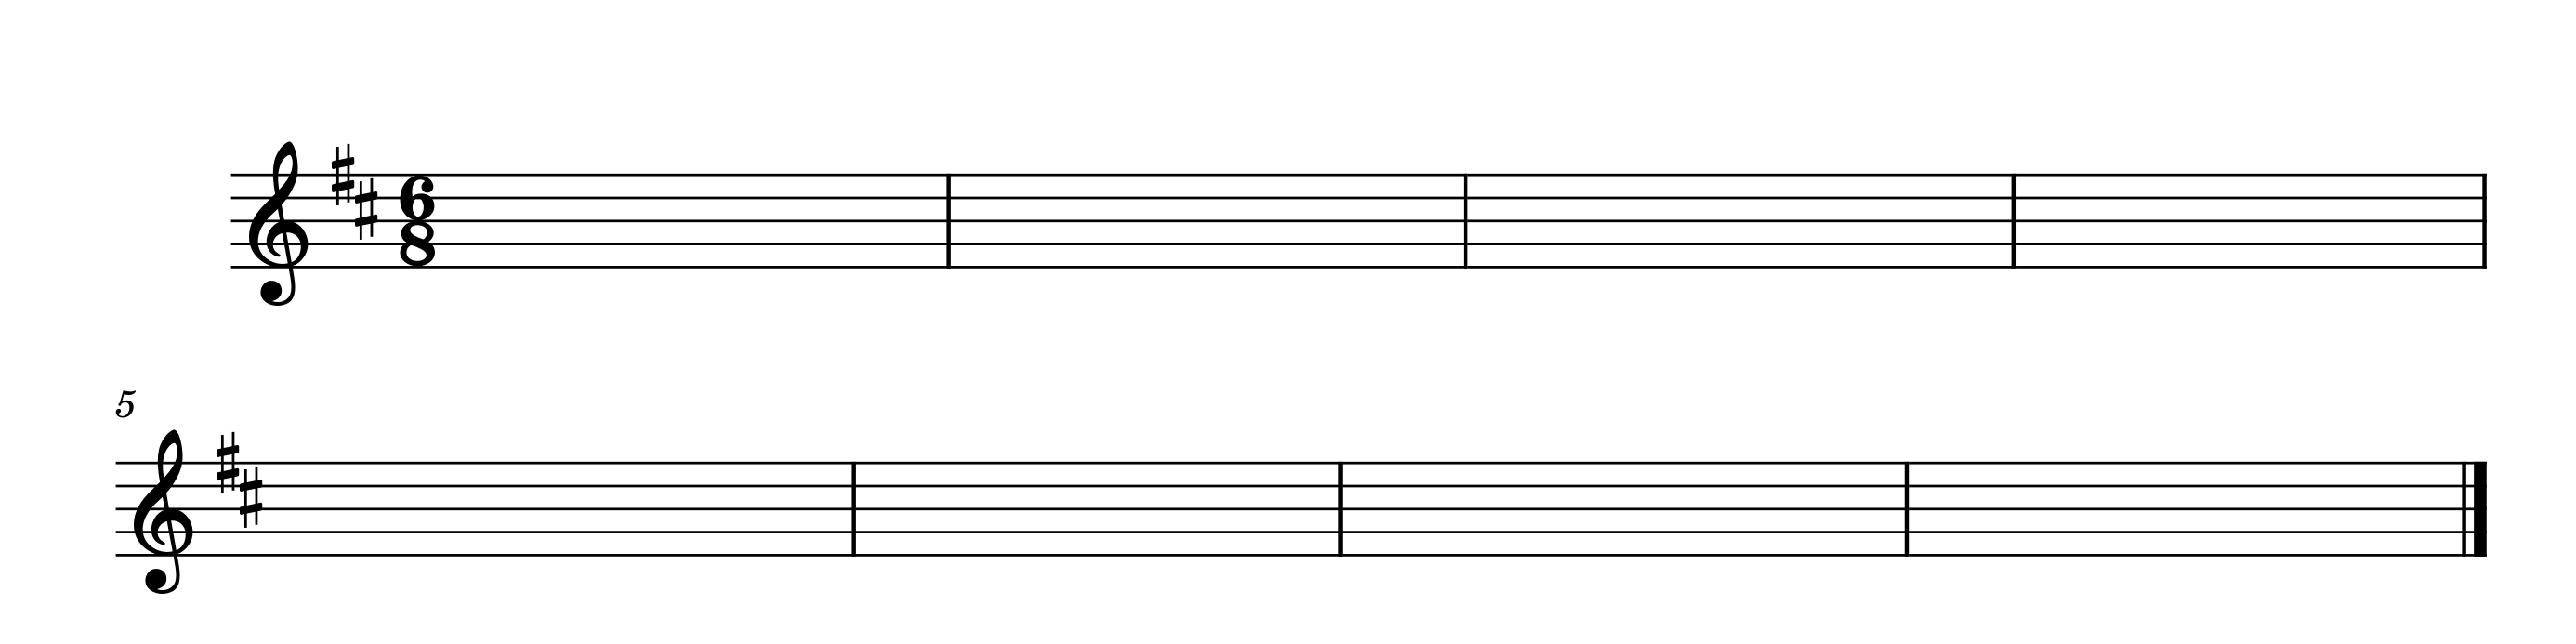
\includegraphics[scale=0.90]{images/Seikilos-1.png}
\caption{Transcrición a notación moderna do epitadio de Seikilos}
\label{transcricion}
\end{figure}
